
\chapter{Processo de Reengenharia}

%Este capítulo fala de \gls{stemmer}s. Mas não esquecer os \Gls{lematizador}es

\section{Sistemas AS-IS}
\subsection{Descrição da Arquitetura/tecnologias utilizadas}
\subsubsection{Tecnologias e Plataformas}
\par Neste ponto serão descritas as tecnologias e plataformas utilizadas ao longo deste trabalho, tais como XAMPP, Laragon, Visual Studio Code.
\par Para a realização deste projeto foram utilizadas as plataformas e tecnologias requeridas pela empresa para facilitar a implementação e integração do projeto, e para tal foi necessário proceder à sua aprendizagem.
\par De seguida vão ser descritas de forma sucinta as tecnologias e plataformas utilizadas ao longo do projeto.\newline


\textbf{XAMPP}

O XAMPP é formado por um pacote que inclui, base de dados MySQL, servidor web Apache e interpretadores para as linguagens de script. É essencialmente utilizado pelos desenvolvedores que pretendem criar um servidor web local no seu próprio computador, com a finalidade de realizar testes sem necessitar de acesso à rede. (Friends, 2018).\newline


\textbf{Visual Studio Code}

O VsCode é um editor de código-fonte simplificado com suporte para operações de desenvolvimento como \textit{debugging}, execução de tarefas e controlo de versões.\newline % vs code FAQ - https://code.visualstudio.com/docs/supporting/FAQ

\quad \textbf{Xdebug}

\quad O Xdebug é uma extensão para PHP que fornece uma variedade de recursos para melhorar a experiência de desenvolvimento de PHP. (Derick Rethans,2020).\newline


\textbf{Laragon}

O Laragon é uma maneira rápida e fácil de criar um ambiente de desenvolvimento isolado no Windows. Inclui Mysql, PHP Memcached, Redis, Apache.(Keycdn,2015).\newline

% keycdn https://www.keycdn.com/blog/web-development-tools
\subsection{Identificação das lacunas/melhorias a realizar}
\section{Sistemas TO-BE}
\subsection{Requisitos Funcionais}
\subsection{Requisitos técnicos e restrições ao desenvolvimento}





%O \acrfull{http} é um protocolo baseado em \acrshort{tcp}.

\section{Figuras}

Ao contrário do Word, o \LaTeX{} usa um mecanismo de colocação de figuras e tabelas em que estas
flutuam ao longo das páginas de acordo com a necessidade/disponibilidade em termo de espaço vertical.
Assim, não devem usar frases como ``na figura acima'', ou ``na figura abaixo'', mas fazer referências:
``tal como se pode observar na Figura~\ref{fig:1}.''

\begin{figure}[htb]
    \centering
    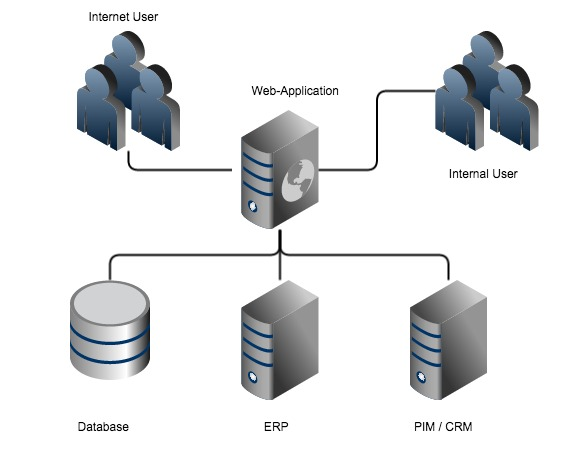
\includegraphics[width=0.8\linewidth]{images/sample}  % largura percentual
    \caption{Esta é a legenda da figura}
    \label{fig:1}
\end{figure}

O mesmo acontece com as tabelas, como se pode ver na Tabela~\ref{tab:1}.

\begin{table}[htb]
    \centering
    \begin{tabular}{ccccc}
        \toprule
        \textbf{A} & \textbf{B} & \textbf{C} & \textbf{D} & \textbf{Total} \\
        \midrule
          1 & 2 & 3 & 4 & 10  \\
          2 & 3 & 4 & 5 & 14  \\
          3 & 4 & 5 & 6 & 18  \\
          4 & 5 & 6 & 7 & 22  \\
         \bottomrule
    \end{tabular}
    \caption{Legenda da tabela.}
    \label{tab:1}
\end{table}

Para a inclusão de código, usa-se algo semelhante. Veja-se a Listagem~\ref{lst:1}.

\begin{lstlisting}[language={[sharp]c},
                   caption={Método para contar o número de elementos numa lista iguais a uma determinada string.},
                   label=lst:1]
   public int count(string x) {
       return items.Select( y => y == x ).Count();
   }
\end{lstlisting}
